% CAPITULO 1-------------------------------------------------------------------

\chapter{TAREFA 1: METODOLOGIA DE DESENVOLVIMENTO}
\label{sec:tarefa1}

Metodologias de desenvolvimento são uma série de técnicas aplicadas durante um projeto de desenvolvimento de software com o objetivo de auxiliar na realização do projeto. Devido a natureza complexa da tarefa, a ausência de uma metodologia pode transformar um projeto de software em um verdadeiro caos. No início se utilizavam o que chamamos hoje de metodologias tradicionais, mais burocráticas e sequenciais, a  exemplo do que era feito na engenharia. Com o tempo começaram a ganhar espaço as metodologias ágeis, voltadas para projetos mais dinâmicos, melhorando a resposta a mudanças durante o projeto.

\section{Metodologia Tradicionais}
\label{sec:tradicional}

Quando a computação surgiu, os programas desenvolvidos eram criados para resolver problemas pontuais, como ler informações do disco ou realizar cálculos matemáticos. Com o crescimento da tecnologia, surgimento de sistemas operacionais e sistemas corporativos, criou-se a necessidade de gerenciar estes grandes projetos. As metodologias tradicionais de desenvolvimento apareceram como uma resposta a essa necessidade.

Na criação destas metodologias, os projetos de engenharia foram utilizados como referência. Portanto as metodologias tradicionais seguem o paradigma de coletar requisitos, desenhar, construir e dar manutenção. Sequencialmente. Por isso a primeira metodologia utilizada foi a metodologia em cascata, ou waterfall. Devido a óbvia limitação com relação a mudanças nos requisitos, logo surgiram as metodologias Unified Process (processo unificado) e Espiral.

A metodologia de processo unificado agregava diversas técnicas de construção de software, utilizando diagramas UML. Nesta metodologia, as fases não eram finalizadas antes do início da próxima fase. As fases eram sobrepostas umas as outras, permitindo com que alterações ocorressem durante o projeto. Já a metodologia em espiral era semelhante a metodologia em cascata. Mas uma vez finalizado o desenvolvimento, voltava-se para o início para que novas funcionalidades fossem agregadas ao projeto.

\begin{figure}[H]
    \centering
    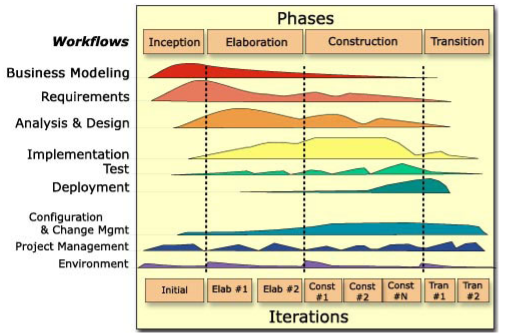
\includegraphics[width=0.7\linewidth]{dados/figuras/metodologia}
    \caption{Ciclo do processo unificado}
    \label{fig:metodologia}
\end{figure}


\section{Métodos Ágeis}
\label{agil}

Com a disseminação da computação e a utilização de sistemas para diversas atividades, surgiu a necessidade e tornar o processo de criação de softwares mais dinâmico. O momento chave para a criação dos chamados métodos ágeis foi a criação do Manifesto para Desenvolvimento Ágil de Software, em 2001. A partir do manifesto a ideia de que um software de qualidade e, principalmente, a satisfação do cliente só seriam atingidos com metodologias mais ágeis e menos restritivas ganhou força. Diversas técnicas surgiram, entre elas a programação extrema, o Scrum e o Kanban.

A programação extrema, ou eXtreme Programming (XP), é o oposto aos longos ciclos de desenvolvimento das metodologias tradicionais. O processo XP é caracterizado por ciclos de desenvolvimento curtos, planejamento incremental, feedback e revisões contínuas, além de um design em constante evolução. Com essas características, os desenvolvedores conseguem responder as mudanças com muito mais qualidade. Entre outras técnicas a XP introduziu a técnica de programação em pares, onde dois programadores trabalham em apenas um computador), a técnica de refatoração (melhorias no código, mesmo que ele esteja funcionando) e a simplificação do design (colocando a enfase no design da solução mais simples para resolver o problema).

O Scrum é um dos métodos ágeis mais conhecidos e utilizados. Ele é um processo iterativo e incremental de desenvolvimento de software. As atividades a serem desenvolvidas no projeto ficam alocadas em um conjunto chamado backlog – nesse caso o backlog do produto. O trabalho é dividido em iterações chamadas sprints. As tarefas que serão executadas em um determinado sprint são definidas em uma reunião de planejamento, sendo movidas do backlog do produto para o backlog do sprint. O Scrum também define reuniões diárias, de apenas 15 minutos, onde todos devem relatar o andamento e se possuem alguma dificuldade que pode bloquear o processo.

\begin{figure}[H]
    \centering
    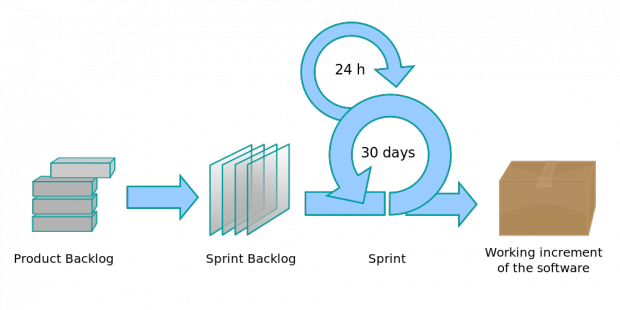
\includegraphics[width=0.7\linewidth]{dados/figuras/agil}
    \caption{Processo Scrum}
    \label{fig:agil}
\end{figure}

Outra metodologia ágil bastante utilizada é o Kanban. Originalmente criado para a indústria, o Kanban se baseia em três princípios básicos: visibilidade do que deve ser feito, limite do trabalho em execução e fluxo de trabalho melhorado. Um quadro com as tarefas é utilizado para dar a visibilidade e controlar o andamento das tarefas. Pelo dinamismo do Kanban, ele é apropriado para projetos onde as prioridades são constantemente alteradas.
\cite{motodologia}

\section{Metodologia de Trabalho Sugerida}

Para a empresa de roupas T-Shirt a metodologia de trabalho escolhida será a metodologia ágil, abaixo serão mencionados algumas das principais vantagens da escolha desta metodologia.

\textbf{1. Mais independência e produtividade para a equipe}

Estruturas ultrapassadas inibem o pensamento criativo e impactam negativamente na produtividade de uma equipe de TI. Quando as Metodologias Ágeis são utilizadas, há uma otimização do tempo e rentabilidade da gestão, visto que não será necessário se preocupar com contratos e documentações extensas e complicadas, ou com ferramentas rígidas que impedem uma resposta rápida para imprevistos.

Assim, a equipe torna-se mais independente e com um melhor preparo para lidar com as resoluções de problemas. Dessa maneira, eles não perdem mais tempo como perdiam utilizando as metodologias tradicionais, e aumentam a produtividade.

\textbf{2. Melhorias na comunicação}

Essas metodologias visam manter um bom relacionamento com os desenvolvedores e clientes. Para que isso aconteça, tudo é pensado para facilitar e otimizar este diálogo, sendo que muitos adeptos preferem as conversas pessoais, a outras formas de comunicação.

Além do mais, essa técnica conta com uma boa prática de feedback. Isso significa que o desenvolvedor sempre estará por dentro das informações do cliente e do código. Essa informação se dá por testes que apontam erros e possíveis formas de melhorias.

\textbf{3. Melhor definição do objetivo}

Com uma maior integração, colaboração do cliente, feedback e softwares, torna-se possível ter uma melhor definição do objetivo, visto que todas as questões principais de uma gestão de TI passam a ser mais claras.

Dessa forma, as Metodologias Ágeis garantem uma nova abordagem, sendo mais adaptada às constantes mudanças que são presenciadas atualmente. Tudo isso colabora para se fazer um planejamento mais eficaz para a gestão de TI, já que os projetos dessa área precisam de soluções muito rápidas e um bom preparo para imprevistos.

\textbf{4. Melhor atendimento ao cliente}

As Metodologias Ágeis acreditam que a atenção deve ser focada nas pessoas, uma vez que são elas que tornam possível que os processos e projetos aconteçam. Por causa disso, fazem de tudo para impulsionar os agentes relacionados aos projetos, principalmente os clientes. O atendimento será melhor, porque a busca pela satisfação do consumidor estará em primeiro lugar.

Como podemos observar, as Metodologias Ágeis proporcionam muitos benefícios para a gestão de TI. Por isso, sua utilização torna-se um importante investimento a ser feito pela empresa T-Shirt.